\chapter{物理仿真和近场动力学方法(PDM)介绍}

\section{物理仿真之基本原理}
绝大多数物理仿真遵循相同的基本流程,都可以认作是牛顿第二定律 $F = Ma$ 的不同形式的体现。如图\ref{fig_physically_based_animation} 所示:
\begin{figure}[htbp!]
  \centering
  \captionsetup{justification=centering}
  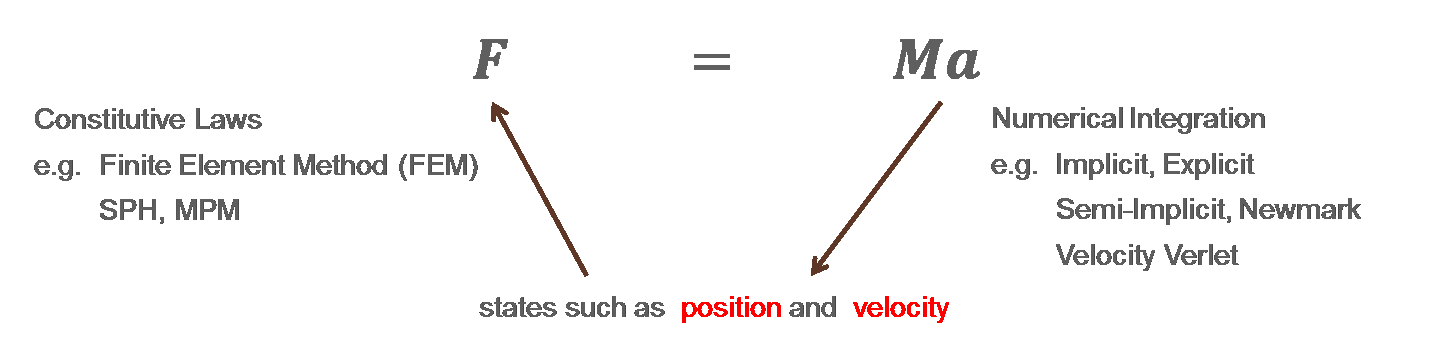
\includegraphics[width=\linewidth]{chap/image/physically_based_animation}

  \caption{\label{fig_physically_based_animation}
           物理仿真动力学循环示意图。物体所受内外力、加速度、以及物体状态构成动力学循环三角。
          }
\end{figure}

在物理仿真中,需要关注三个核心的动力学要素:物体所受内外力,加速度,以及物体的状态。从物体的当前所处状态,即物体的位置和速度信息,来推导物体当前各部分所受力,所涉及的是物理仿真中最为关键的部分——动力学本构模型。通俗而言,本构模型描述的是材料的形变与动力学行为之间的关系,一般也称为内力模型。常见的本构模型包括用来描述固体运动的有限元方法(FEM)、用来描述流体运动的光滑粒子动力学(SPH)\textcolor{blue}{(M\"{u}ller et al. )\parencite{Muller2003}}、 以及适合对雪进行建模的物质点法(MPM)\mycite{Stomakhin}{2013}等。关于本构模型的一般性介绍,将呈现于章节\ref{constitutive_model}。

根据物体所受力 $F$,则可以根据牛顿第二定律直接获得物体的加速度 $a$。 而从物体所受加速度进一步推导得到物体的当前状态,所涉及到的则是离散时间积分算法。离散积分算法的作用是在给定时间步 $\Delta t$ 下,物体的状态将以何种方式进行更新。不同的离散时间积分算法对物理仿真的稳定性、精确性和效率有重大影响,本文将在\ref{numerical_method} 小节详细阐述。

可以看到,物体所受内外力、加速度、以及物体状态构成了一个动力学循环三角,并通过牛顿第二定律、本构模型、数值积分算法进行衔接。绝大部分仿真算法都是采用关键帧(key frame)的形式,因为在复杂场景中,物体的运动几乎不可能以解析的形式来表达,因此需要随着时间步而不断向前迭代,以此获得物体完整的运动状态序列。

\section{碎裂仿真之基本流程}
碎裂仿真是物体仿真的一个具体特化,但相对于传统仿真更具复杂性。其原因不仅在于碎裂模式的多样化,更在于在碎裂发生的情况下,物体本身拓扑表达的变化,将导致物体单元体或节点的数量也将发生改变。典型的碎裂仿真流程如图
\ref{fig_fracture_animation_pipeline}总结:
\begin{figure}[htbp!]
  \centering
  \captionsetup{justification=centering}
  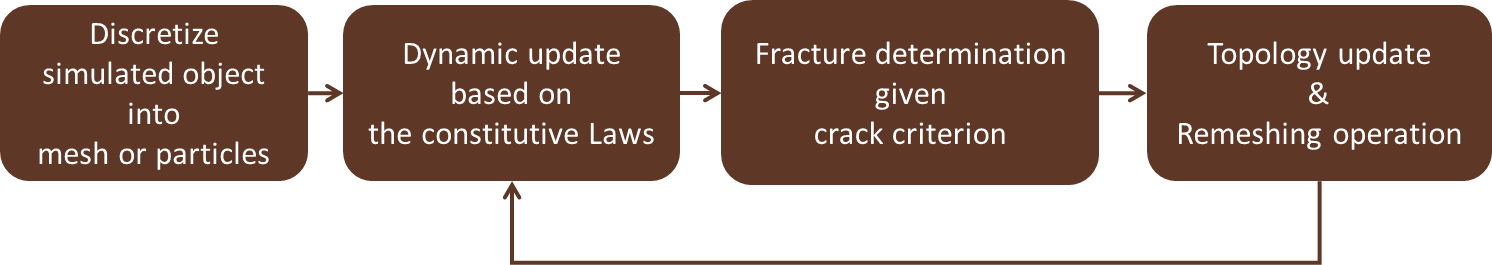
\includegraphics[width=\linewidth]{chap/image/fracture_animation_pipeline}

  \caption{\label{fig_fracture_animation_pipeline}
           碎裂仿真的基本流程。主要分为四个关键步骤,分别是物体离散、动力学更新、碎裂发生判断,拓扑更新。
          }
\end{figure}

从图\ref{fig_fracture_animation_pipeline}可以看出,碎裂仿真主要包含四个步骤。

第一个步骤是在动力学仿真开始前,需要以合适的方式对物体进行离散,由于计算资源是有限的,因此不可能以无限微分的方式来对物体进行建模计算,而只能用有限的状态集表示。一般而言,离散方式和本构模型直接挂钩。对于传统基于网格的方法,如 FEM,通常将物体离散成四面体或六面体体网格,对于薄壳体则离散成三角面片网格\mycite{Pfaff}{2014}。而对于无网格方法,则通过粒子集合来表示物体\mycite{Pauly}{2005}。

第二个步骤是在物体已知状态下,通过动力学本构模型和数值积分算法来对物体的状态进行更新,这一步骤是所有物理仿真所必须的。

第三个步骤和第四个步骤是根据给定的碎裂标准和阈值判断物体中的某些节点是否应该发生碎裂,碎裂模型一般建立在已有的本构模型之上,本文将在章节\ref{fracture_model_section}进行一般性介绍。如果判断物体部分节点发生碎裂,则往往需要对拓扑进行更新。对于有网格方法,在必要情况下,还需要对拓扑网格进行 remeshing 操作以对网格进行精化。在拓扑更新完之后,将进入下一个循环的动力学更新。关于本文工作所用的碎裂模型和拓扑更新方式,将在第四章进行阐述。

\section{本构模型泛述}
\label{constitutive_model}
在图形学领域及工程材料领域,一般研究的是物质的宏观运动。但实际上物质都是由大量分子组成的,分子间的真空区尺度远大于分子本身,并且每个分子在无休止的做不规则运动,相互间经常碰撞,交换着动量和能量。因此物质的微观结构和运动无论在时间上还是空间上都充满着不均匀性、离散性和随机性。而另一方面人们用仪器测量或者用肉眼观察到的物质宏观结构和运动却又明显呈现出均匀性、连续性和确定性。这两种特性如此之不同却又和谐统一地表现于物质之中。研究物体的宏观运动存在两种不同的途径,一种是基于统计物理的方法,其直接从分子和原子的运动出发,采用统计平均的方法建立宏观物理量满足的方程,但这种方法迄今为止还不完善。另一种方法则是以连续介质为假设,认为物质连续地充满物体所在的整个空间,构成物体的物质单元或质点在微观上认为充分大,但在宏观上又被认为足够小。其具有的宏观物理量(质量、速度、力)满足一切都应遵循的物理定律及物理性质,例如牛顿定律、质量守恒定律和能量守恒定律等。这一假设已经被学术界广为采用,并且在揭示物质材料的动力学性质上已经取得巨大成功。

现有的本构模型几乎都基于连续介质假设,典型如描述固体的连续介质力学\mycite{Eduardo}{2013}和描述流体的Navier-Stokes方程。本构模型描述的是在连续介质假设下,物体某微元根据自身状态以及周围状态所作出的反应,其一般以解析形式表达在外力和边界条件作用下,物体产生的内力将如何反抗相应的形变行为。

本文工作所采用的近场动力学理论和连续介质力学中的线性模型在理论上是对等的,所以下面将对连续介质力学的理论基础尤其是线性模型做必要介绍。

在连续介质力学中,用来表示物体形变的关键变量是形变梯度 $\F \in \textbf{R}^{3\times3}$,其定义为

\begin{equation}
\F \equiv \frac{\partial(\boldmath{x}, \boldmath{y}, \boldmath{z})}{\partial(\X, \Y, \Z)}
=
\left(
  \begin{array}{ccc}
    \frac{\partial\boldmath{x}}{\partial\X}& \frac{\partial\boldmath{x}}{\partial\Y} & \frac{\partial\boldmath{x}}{\partial\Z} \\
    \frac{\partial\boldmath{y}}{\partial\X}& \frac{\partial\boldmath{y}}{\partial\Y} & \frac{\partial\boldmath{y}}{\partial\Z} \\
    \frac{\partial\boldmath{z}}{\partial\X}& \frac{\partial\boldmath{z}}{\partial\Y} & \frac{\partial\boldmath{z}}{\partial\Z} \\
  \end{array}
\right)
\end{equation}

其中 $\X, \Y, \Z$ 表示的是形变之前的位置,亦即参考/未形变空间(reference/undeformed space)的位置。$\boldmath{x}, \boldmath{y}, \boldmath{z}$ 则表示形变后的位置,亦即在世界空间(world space)的位置。在形变梯度的基础上,可以进一步定义格林应变张量 $\E \in \textbf{R}^{3\times3}$(Green strain tensor),即

\begin{equation}
\E = \frac{1}{2}\left(\F^{T}\F - \textbf{I}\right)
\end{equation}

不难看出,格林应变张量是关于形变的二次函数,也即其在几何上是非线性的,并且具有旋转不变性。使用格林应变张量的模型(e.g. Stvk Model)在求解上将更为复杂,可以对其进行线性近似(linear approximation),得到柯西应变张量(Cauchy strain tensor)

\begin{equation}
\mathbf{\epsilon} = \frac{1}{2}(\F^T + \F) - \textbf{I}
\end{equation}

柯西应变张量是关于形变的线性函数,在求解上也较为简便。但其并不具有旋转不变性,也即当只发生刚体的旋转时,将会产生实际上并不应该存在的力(ghost force)。为克服此一问题,更多的是采用共旋线性模型(Corotated Linear Model),其基本原理是对形变梯度 $\F$ 进行极化分解(polar decomposition),去除其旋转分量。如下,

\begin{equation}
\begin{aligned}
\F & = \textbf{RS} \\
\mathbf{\epsilon}_c & = \textbf{S} - \textbf{I}
\end{aligned}
\end{equation}

上述公式中 $\textbf{R}$ 表示旋转部分,$\textbf{S}$ 则为形变部分,其是对称张量。在形变张量 $\mathbf{\epsilon}$ 的定义中,可以看到旋转部分 $\textbf{R}$ 被舍弃,而只与形变相关,因此共旋线性模型具有旋转不变性。本文工作所用本构模型将基于全新的近场动力学理论,其是连续介质力学中的线性模型推导而来,并且同样具有旋转不变性,本文将在第三章进行详细阐述。

虽然在几何上对于形变的度量具有线性和非线性之分,但在材质模型的选择上上,大多数工作都是采用线性模型来计算能量密度 $\mathbf{\psi} $,应力张量$\mathbf{\sigma}$,具体如下:

\begin{equation}
\begin{aligned}
\mathbf{\Psi} = &\frac{1}{2}\mathbf{\epsilon}^T\textbf{C}\mathbf{\epsilon}\\
\mathbf{\sigma} = &\textbf{C}\mathbf{\epsilon}
\end{aligned}
\end{equation}

其中考虑形变张量$\mathbf{\epsilon}$和应力张量$\mathbf{\sigma} $的对称性,将其重整为向量形式,

\begin{equation}
\begin{aligned}
\mathbf{\epsilon} &= \left(
                      \begin{array}{ccccccc}
                         \mathbf{\epsilon}_{xx}\quad
                         \mathbf{\epsilon}_{yy}\quad
                         \mathbf{\epsilon}_{zz}\quad
                         \mathbf{\epsilon}_{yz}\quad
                         \mathbf{\epsilon}_{xz}\quad
                         \mathbf{\epsilon}_{xy}
                      \end{array}
                    \right)^T\\
\mathbf{\sigma} &= \left(
                      \begin{array}{cccccc}
                         \mathbf{\sigma}_{xx}\quad
                         \mathbf{\sigma}_{yy}\quad
                         \mathbf{\sigma}_{zz}\quad
                         \mathbf{\sigma}_{yz}\quad
                         \mathbf{\sigma}_{xz}\quad
                         \mathbf{\sigma}_{xy}
                      \end{array}
                  \right)^T
\end{aligned}
\end{equation}

最后,$\textbf{C}$ 被称为物质材质矩阵(material property matrix),定义为

\begin{equation}
\textbf{C} = \left(
               \begin{array}{cccccc}
                 \kappa + (4\mu/3) & \kappa - (2\mu/3) & \kappa - (2\mu/3) & 0 & 0 & 0 \\
                 \kappa - (2\mu/3) & \kappa + (4\mu/3) & \kappa - (2\mu/3) & 0 & 0 & 0 \\
                 \kappa - (2\mu/3) & \kappa - (2\mu/3) & \kappa + (4\mu/3) & 0 & 0 & 0 \\
                 0 & 0 & 0 & \mu & 0 & 0 \\
                 0 & 0 & 0 & 0 & \mu & 0 \\
                 0 & 0 & 0 & 0 & 0 & \mu \\
               \end{array}
             \right)
\end{equation}
上式中 $\kappa$ 和 $\mu$ 分别表示体积模量和剪切模量。

在给定离散框架下(如 FEM),则可以相应计算形变梯度 $\textbf{F}$,进而获得应力张量 $\mathbf{\sigma}$,最终可以通过加权平均的方式算得作用力,并施加到离散模型的各个节点之上。

\section{碎裂模型泛述}
\label{fracture_model_section}

碎裂本质上是材料一种结构屈服和能量释放行为,在物理仿真中通过专门的碎裂模型来描述。碎裂模型通常直接建立在本构模型之上,其主要功能在于两点。第一,判断碎裂是否发生。第二,判断裂纹生长的方向。碎裂模型一般是在通过本构模型计算已得的物理量的基础之上,构建一个衡量碎裂的中间标准物理量来计算碎裂是否发生以及碎裂方向。

\begin{figure}[!htb]
  \centering
  \captionsetup{justification=centering}
  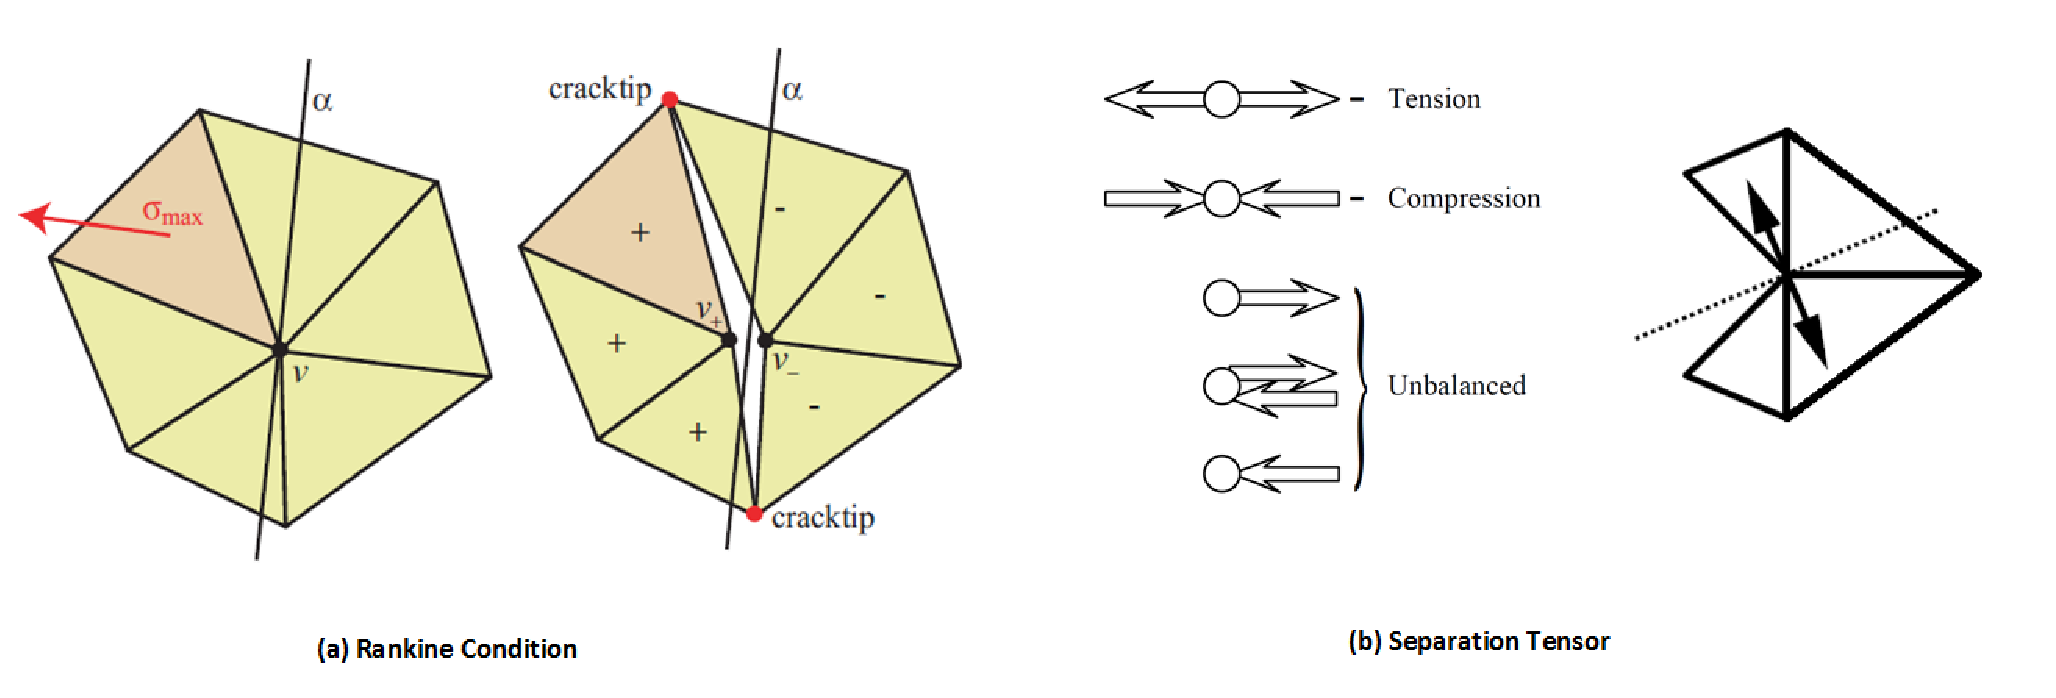
\includegraphics[width=\linewidth]{chap/image/fracture_model}

  \caption{\label{fracture_model}
           碎裂模型示意图。左边为Rankine Condition,右边为 Separation Tensor。图片分别取自\textcolor{blue}{(M\"{u}ller et al. )\parencite{Muller2004}} 和\textcolor{blue}{(O'Brien et al. )\parencite{OBrien1999}}。
          }
\end{figure}

最常用的碎裂模型包括 Rankine Condition,其基本原理是计算物质节点的主应力大小 $\mathbf{\sigma}_{max}$ 以及主应力方向 $\textbf{n}_{max}$,如果 $\mathbf{\sigma}_{max}$ 超出阈值则认定碎裂发生,并且裂纹方向即为 $\textbf{n}_{max}$。 应用此碎裂模型的典型工作包括\textcolor{blue}{(M\"{u}ller et al.)\parencite{Muller2004}}。 但 Rankine Condition 的缺陷是即使某一方向受力较大,也会导致碎裂发生,而事实上碎裂是由相互抵消的力(挤压或者撕扯)的大小而决定的。因此,另一种常用的碎裂模型是 Separation Tensor\textcolor{blue}{(O'Brien et al.)\parencite{OBrien1999}} ,其计算的是相互抵消的应力最大的力大小和方向,因此克服了 Rankine Condition 的缺陷,不过其在计算上相对要较为复杂。两种碎裂模型的示意图如图\ref{fracture_model} 所示。

对于质点弹簧系统或者无网格中的方法,其作用关系一般是通过粒子与粒子之间的连接而决定的。因此,在碎裂模型上往往不涉及裂纹生长的方向,而是可以直接通过去除粒子之间的相互作用力来体现。在无网格框架中,最常用的碎裂模型是临界伸长量(critical stretch)。假设粒子之间通过弹簧相连,如果其伸长比例超过阈值,则断裂发生。本文所用的碎裂模型基于 critical stretch,但对其有所改进,具体在第四章详述。

\section{离散时间积分}
\label{numerical_method}
在章节\ref{related_work}所阐述的有网格方法和无网格方法本质上是在空间上对物体进行离散化,而求解物体的运动还需要在时间维度上进行离散化,在时间维度上的离散化数值积分被称为离散时间积分。精确性(accuracy)和稳定性(stability)是衡量离散时间积分算法优劣的两大指标,其中精确性衡量的是离散积分的解与连续解之间的误差,而稳定性衡量的是误差是否会随时间累积。关于数值积分的详细介绍,参见\mycite{Michael}{1997}。

离散时间积分决定以何种方式来对系统中的状态进行更新。在大多数系统中,通常需要关心的状态更新是位置 $\textbf{x}$ 和速度 $\textbf{v}$。 对于无网格方法,$\textbf{x}$ 和 $\textbf{v}$ 被直接赋予到粒子之上。而对于有网格方法,虽然整体的物理动力学计算是基于网格中的单元体的,但实际上单元体在拓扑上仍然由节点/顶点连接而成,所以最后的计算结果仍然将会以加权平均的方式施加到各个顶点之上。

假设某粒子 $i$ 所受内力为 $\fin$,所受外力为 $\fex$,速度为 $\vi$,位置为 $\xii$,质量为 $m_i$。则根据速度的定义以及牛顿第二定律,得到:
\begin{equation}
\label{eq1}
\left\{ \begin{array}{l}
\frac{\textrm{d}\xii}{\textrm{d}t} = \dot{\xii}=\vi\\
\frac{\textrm{d}\dot{\xii}}{\textrm{d}t} = \frac{\textrm{d}\vi}{\textrm{d}t}=\frac{\fin + \fex}{m_i}
\end{array} \right.
\end{equation}
注意在上述公式中 $\xii$ 和 $\vi$ 都是关于时间的函数,离散时间积分是通过 $\xii(t_0)$ 和 $\vi(t_0)$ 来求解 $\xii(t_0 + \Delta t)$ 和 $\vi(t_0 + \Delta t)$的状态。

最常见的两种时间积分算法分别是显式欧拉积分(explicit Euler integration)和隐式欧拉积分(implicit Euler integration)。在下面小节中,我们将分别进行介绍。

\subsection{显式欧拉积分}
\label{explicit_euler_method}

\begin{figure}[!htb]
  \centering
  \captionsetup{justification=centering}
  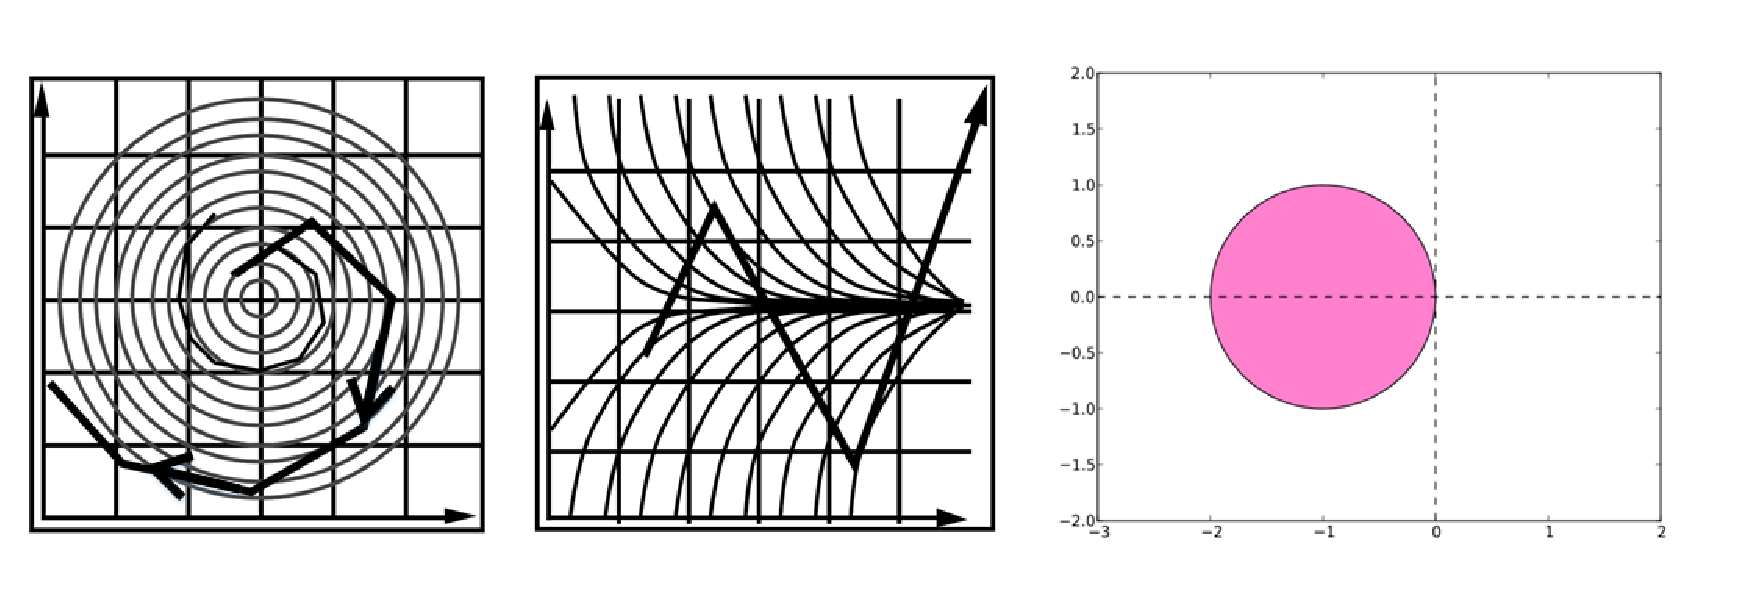
\includegraphics[width=\linewidth]{chap/image/explicit_method}

  \caption{\label{explicit_method}
           显式欧拉积分。随着仿真的进行,误差将很容易累积,从而导致仿真系统崩溃。粉色区域为绝对稳定区域。图片取自\mycite{Witkin}{1997}
          }
\end{figure}

显式积分亦称前向欧拉积分(forward Euler method),其思想来源于在 $t_0$ 时刻的一阶泰勒展开 $f(t_0 + \Delta t) \approx f(t_0) + \dot{f}(t_0)\Delta t$,$t_0 + \Delta t$ 时刻的状态完全直接由 $t_0$ 时刻的状态决定。具体而言,
\begin{equation}
\left\{ \begin{array}{l}
\vi(t_0+\Delta t) = \vi(t_0)+\frac{\fin(t_0) + \fex(t_0)}{m_i}\Delta t\\
\xii(t_0+\Delta t) = \xii(t_0)+\vi(t_0)\Delta t
\end{array} \right.
\end{equation}

上式左边皆为 $t_0 + \Delta t$ 时刻的待求解物理量,而右边则为 $\Delta t$ 时刻的已知物理量。显式欧拉积分是最容易实现的离散积分方式,并且可以直接并行化。在数值准确性上其具备一阶数值精度,但稳定性较差。当时间步长 $\Delta t$ 较长时,容易累积误差而致使整个仿真系统崩溃,如图\ref{explicit_method}。 因此使用显式积分的仿真系统往往需要设置较小的时间步,并且同时添加阻尼力保证仿真的稳定性。可以进行些许修改从而一定程度上改善其稳定性:
\begin{equation}
\left\{ \begin{array}{l}
\vi(t_0+\Delta t) = \vi(t_0)+\frac{\fin(t_0) + \fex(t_0)}{m_i}\Delta t\\
\xii(t_0+\Delta t) = \xii(t_0)+\vi(t_0 \textcolor{red}{ + \Delta t})\Delta t
\end{array} \right.
\end{equation}
这种形式的数值积分算法被称为半隐式欧拉积分(Semi-implicit Euler integration)。本文工作大部分都采用此种形式的积分算法,具体计算流程可用如下伪码表示:\\

\noindent\fbox{
\parbox{0.6\textwidth}{

\textcolor{green}{//initialization}\\
(1) \textbf{forall} particles $i$ \\
(2) \qquad initialize $m_i$ and other necessary info\\
(3) \qquad $\xii \leftarrow \xii(t_0)$\\
(4) \qquad $\vi \leftarrow \vi(t_0)$\\
(5) \textbf{endfor}\\
\textcolor{green}{//simulation loop}\\
(6) \textbf{loop}\\
(7) \qquad \textbf{forall} particles $i$\\
(8) \qquad \qquad calculate $\fin$ from constitutive laws\\
(8) \qquad \qquad calculate $\fex$ from boundary conditions\\
(9) \qquad \qquad $\vi\leftarrow \vi + \Delta t\cdot \frac{\fin + \fex}{m_i}$\\
(10) \qquad\qquad $\xii\leftarrow \xii +\Delta t\cdot \vi$\\
(11) \qquad\textbf{endfor}\\
(12) \qquad display the system every $n^{th}$ time\\
(13) \textbf{endloop}
}
}\\

\subsection{隐式欧拉积分}
\label{implicit_euler_method}

\begin{figure}[!htb]
  \centering
  \captionsetup{justification=centering}
  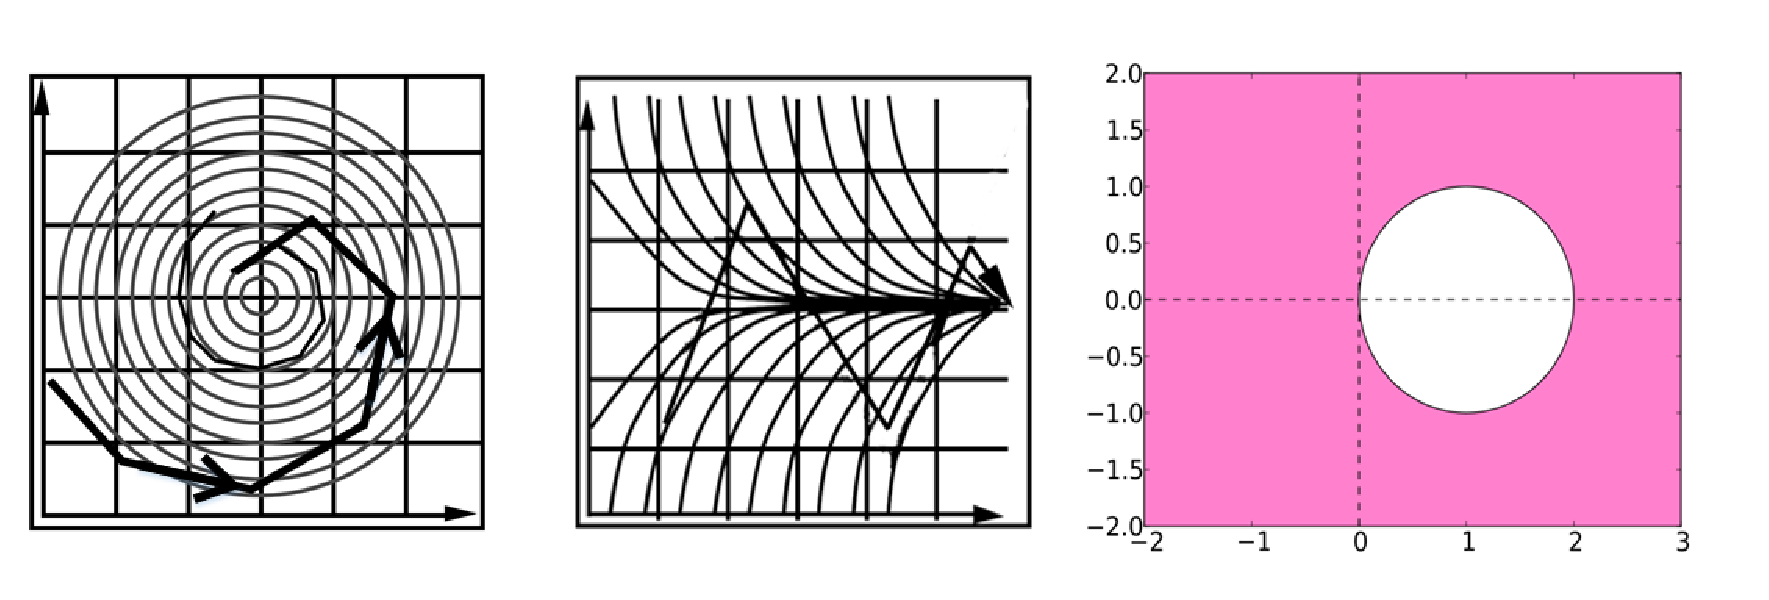
\includegraphics[width=\linewidth]{chap/image/implicit_method}

  \caption{\label{implicit_method}
           隐式欧拉积分。隐式欧拉积分理论上可认为是无条件稳定的,并且自带阻尼效果。图中粉色区域所示为绝对稳定区域。
          }
\end{figure}

不同于显式欧拉积分,隐式欧拉积分理论上可认为是绝对稳定的,其误差并不随时间而积累。一般认为隐式欧拉积分方法自带阻尼效果,其会导致能量的耗散,如图\ref{implicit_method}所示。隐式欧拉积分的思想来源于在 $t_0 + \Delta t$ 时刻的一阶泰勒近似$f(t_0) \approx f(t_0 + \Delta t) - \dot{f}(t_0 + \Delta t)\Delta t$,因此也称之为向后欧拉算法(backward Euler method)。其具体积分形式可写为:
\begin{equation}
\left\{ \begin{array}{l}
\vi(t_0+\Delta t) = \vi(t_0)+\frac{\fin(t_0 \textcolor{red}{+ \Delta t}) + \fex(t_0 \textcolor{red}
                                  {+ \Delta t})}{m_i}\Delta t\\
\xii(t_0+\Delta t) = \xii(t_0)+\vi(t_0 \textcolor{red}{ + \Delta t})\Delta t
\end{array} \right.
\end{equation}

进一步,
\begin{equation}
\label{eqa25}
\left\{ \begin{array}{l}
\Delta \vi = \frac{\fin(t_0 \textcolor{red}{+ \Delta t}) + \fex(t_0 \textcolor{red}
                                  {+ \Delta t})}{m_i}\Delta t\\
\Delta \xii = \left(\vi(t_0) + \Delta \vi\right)\Delta t
\end{array} \right.
\end{equation}

其中 $\Delta \vi = \vi(t_0 + \Delta t) - \vi(t_0)$ 表示速度增量, $\Delta \xii = \xii(t_0 + \Delta t) - \xii(t_0)$ 表示位置增量,$\fin(t_0 \textcolor{red}{+ \Delta t})$ 和 $\fex(t_0 \textcolor{red}{+ \Delta t})$ 分别代表在 $t_0 + \Delta t$ 时刻的内力和外力。一般而言,$\fex(t_0 \textcolor{red}{+ \Delta t})$ 可以直接用 $\fex(t_0)$ 近似,然而 $\fin(t_0 \textcolor{red}{+ \Delta t})$ 则不然。事实上,除非 $\fin(t_0 \textcolor{red}{+ \Delta t})$ 是线性函数,亦即所仿真材料是线性材料,否则在求解时其并非已知。因此如果 $\fin(t_0 \textcolor{red}{+ \Delta t})$ 是非线性函数(即非线性材料),则此时是无法对其进行精确求解的,只能对其进行一阶泰勒近似,亦即
\begin{equation}
\fin(\xii(t_0) + \Delta \xii(t_0),\vi(t_0)+\Delta \vi) = \fin(t_0) +
                                                         \sum\frac{\partial \fin(t_0)}{\partial \xj}\Delta \xj+
                                                         \sum\frac{\partial \fin(t_0)}{\partial \vj}\Delta \vj
\end{equation}

注意在 $t_0 + \Delta t$ 时刻,$\fin$ 是关于$\xii(t_0 + \Delta t)$ 和 $\vi(t_0 + \Delta t)$的函数,通常 $\fin$ 并不和速度相关,所以上式可以进一步简化为

\begin{equation}
\label{eqa27}
\fin(t_0)+ \Delta t) = \fin(t_0) +\sum\frac{\partial \fin(t_0)}{\partial \xj}\Delta \xj
\end{equation}

将式\ref{eqa27}代入\ref{eqa25},并消去 $\Delta \xii$,则可得

\begin{equation}
\Delta \vi = \frac{\Delta t}{m_i}\left[\fin(t_0) + \fex(t_0)\right]
           + \sum\frac{\Delta t^2}{m_i} \frac{\partial \fin(t_0)}{\partial \xj}
             \left(\vj(t_0) + \Delta \vj\right)
\end{equation}

可以看出,上述公式左边是关于粒子 $i$ 的速度增量$\Delta \vi$,而右边则和周围粒子 $j$ 的速度增量 $\Delta \vj$ 相关。所以不同于显式方法,隐式积分方法是没有办法对状态进行单独求解的,而只能进行全局求解。我们需要将其扩充为向量形式,如下

\begin{equation}
\Delta \textbf{v} = M^{-1}\Delta t\left[\textbf{f}^{int}(t_0) + \textbf{f}^{ext}(t_0)\right]
                  + M^{-1}\Delta t^2 \frac{\partial \textbf{f}^{int}(t_0)}{\partial \textbf{x}}
                    \left(\textbf{v}(t_0) + \Delta\textbf{v}\right)
\end{equation}

其中$M$为质量对角矩阵。将上述方程进行重整,可以得到最终形式:

\begin{equation}
\left(\hat{I} - M^{-1}\Delta t^2 \frac{\partial \textbf{f}^{int}(t_0)}{\partial \textbf{x}}\right)\Delta \textbf{v} = M^{-1}\Delta t\left[\textbf{f}^{int}(t_0) + \textbf{f}^{ext}(t_0)\right]
                  + M^{-1}\Delta t^2 \frac{\partial \textbf{f}^{int}(t_0)}{\partial \textbf{x}}\textbf{v}(t_0)
\end{equation}

或

\begin{equation}
\left(M - \Delta t^2 \frac{\partial \textbf{f}^{int}(t_0)}{\partial \textbf{x}}\right)\textbf{v}(t_0 + \Delta t) = \Delta t\left[\textbf{f}^{int}(t_0) + \textbf{f}^{ext}(t_0)\right]
                  + M\textbf{v}(t_0)
\end{equation}

其中 $\textbf{K} = \frac{\partial \textbf{f}^{int}(t_0)}{\partial \textbf{x}}$ 被定义为刚度矩阵(stiffness matrix)。不难看出,在隐式积分算法下,问题最终转化为一个线性系统 $\textbf{Ax} = \textbf{b}$ 问题的求解。对于大规模的线性矩阵求解问题,一般采用迭代法进行求解,如 Jacobi 迭代法或者 Gauss-Seidel 迭代法。其中 Jacobi 迭代法收敛速度较慢,但适于并行,Gauss-Seidel 迭代法则相反。此外,考虑刚度矩阵 $\textbf{K}$ 一般具有对称性,因此更多的是采用预置共轭梯度的办法(PCG)来进行求解,因为具有非常更加快速的收敛特性。并且在具体实现时,刚度矩阵 $\textbf{K}$ 往往不需要显式构造,只需要提供计算 $\textbf{K} \cdot \Delta \textbf{x}$ 的接口,进一步减少存储空间和提高效率。

隐式欧拉积分在 FEM 和其他无网格方法应用都较为普遍,其相对于显式积分方法在稳定性上具有明显优势。虽然隐式方法实现更为复杂,但由于能够对时间步 $\Delta t$ 的限制有所放松,所以最终仿真效率能够领先于显式积分方法。不过由于近场动力学本身的特殊性,其在计算刚度矩阵 $\textbf{K}$ 时相对于一般系统要多出一层复杂度,所以在本工作中,我们只针对规模较小系统尝试隐式欧拉积分,具体原因将在第三章进行说明。


\section{近场动力学方法(PDM)简介}

\subsection{基本特征和形式}
\label{pdm_basic_feature}
在章节\ref{related_work}中已经提及,相对于其他动力学模型,近场动力学的两大基本特点分别是非局域性以及积分形式的表述。

关于粒子之间作用的局域性问题,存在两种截然不同的理论。以经典连续介质力学为代表的局域性理论,认为粒子在微观上只和其直接邻域发生作用,而和其他粒子无关。这一假设在很大程度上对材质进行了简化,却又基本准确描述了材料的动力学行为,因而在工程领域以及图形学领域应用极多。局域性理论的另一个极端则是分子动力学,其认为每一个粒子和其他粒子都能彼此发生作用,而不仅限于其直接邻居。分子动力学在基础物理领域的仿真应用较大,但在倾向于研究宏观运动行为的图形学领域则应用较少。从局域性的观点来看,近场动力学恰好位于两种理论之间,其假定材质中的物质点会和有限半径范围内的邻域发生作用,因此可认作是连接两种理论的桥梁。如图\ref{peridynamics_comparison}所示:

\begin{figure}[htbp!]
  \centering
  \captionsetup{justification=centering}
  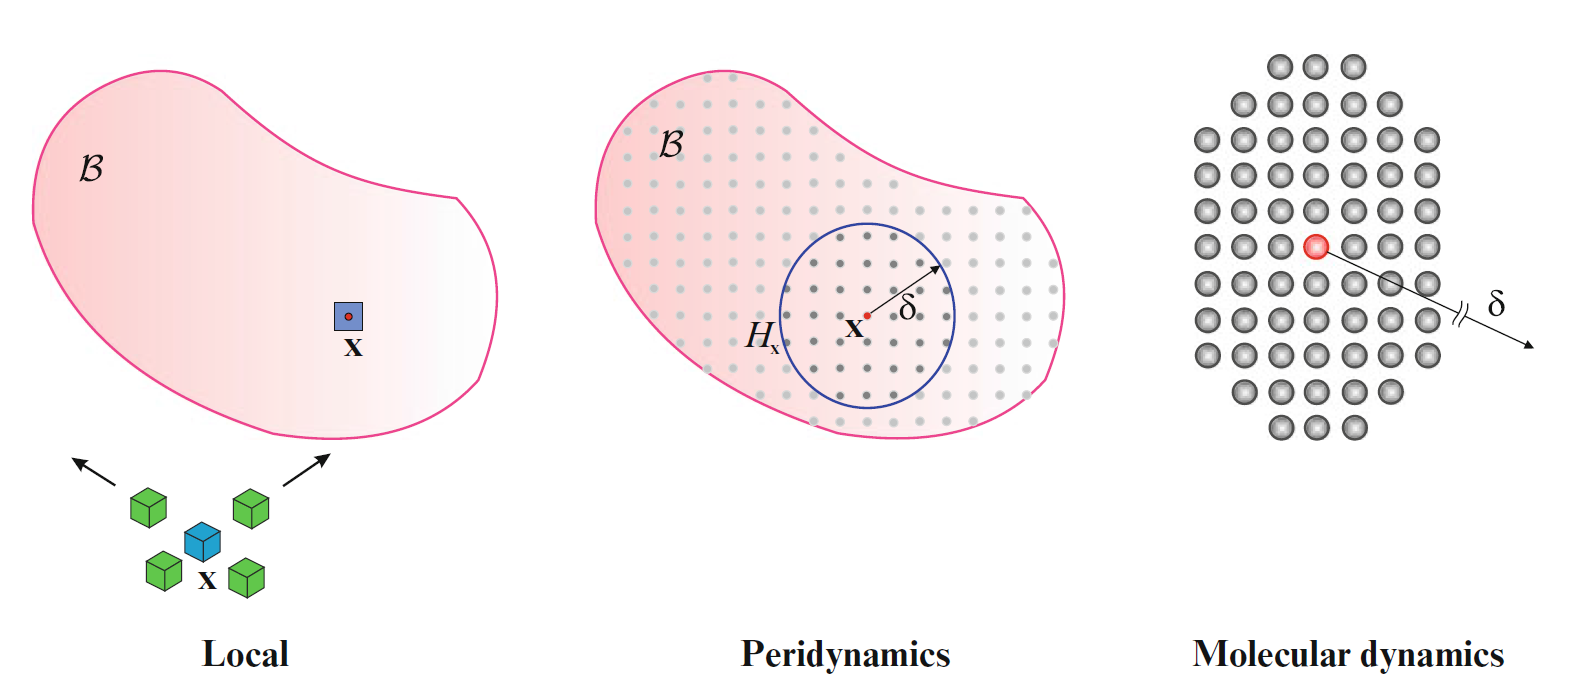
\includegraphics[width=\linewidth]{chap/image/peridynamics_comparison}

  \caption{\label{peridynamics_comparison}
           不同动力学模型的作用域大小对比。左边为局域性理论,粒子只和直接邻域发生相互作用。右边为分子动力学理论,可认定作用半径无限大。而近场动力学位于两者之间,受邻域半径 $\delta$ 范围内的粒子影响。图片取自\mycite{Madenci}{2014}。
          }
\end{figure}

对于近场动力学模型,可以根据图\ref{peridynamics_comparison}中图作更为细致的形式化表述。具体而言,材质中的任何一个物质粒子 $\mathbf{x}$ 将会和其周边半径为 $\delta$ 内的粒子发生相互作用,这一半径 $\delta$ 被定义为\textbf{邻域半径}(horizon),而位于邻域半径 $\delta$ 之内的粒子被定义\textbf{邻域}(family),$H_\mathbf{x}$。对于连续性的材料,在离散化之前,邻域范围内的粒子数量可认定是无穷的。从用粒子来表示物体的观点来看,近场动力学的基本思想和其他无网格方法\textcolor{blue}{(M\"{u}ller et al.)\parencite{Muller2003}}并无大差异,最大的区别在作用半径 $\delta$ 的引入,这也是近场动力学理论被认定为非局域性理论的原由。 \mycite{Silling}{2003}证明,当 $\delta$ 趋向于0 时,近场动力学模型将会退化为经典的连续介质力学。而当 $\delta$ 区域无穷大时,则会成为连续形式的分子动力学理论。

在近场动力学之前,几乎所有的动力学模型都采用的是微分形式的本构方程(governing function)。最为典型的就是在连续介质力学理论中,本构方程一般使用如下形式,

\begin{equation}
\label{fem_governing_function}
\rho\ddot{\mathbf{u}}(\mathbf{x}) = \nabla\cdot\sigma(\mathbf{x})+\mathbf{b}(\mathbf{x})
\end{equation}

其中 $\rho$ 表示粒子的质量密度。$\ddot{\mathbf{u}}$ 为向量,表示粒子的位移。$\mathbf{b}$ 表示粒子所受外力,一般包括重力或者由碰撞导致的外力等。类似的符号表示将同样应用于后续近场动力学的本构方程,后面将不再赘述。在方程\ref{fem_governing_function} 中,最为关键的物理量是 $\nabla\cdot\sigma$,即是二阶应力张量 $\sigma$ 的散度微分,其表示单位体积物体所受的力(力密度)。如前面章节\ref{constitutive_model} 所述, $\sigma$ 的计算尤为关键,其包含物体所有的本构信息。在此,需要尤其注意的是,$\nabla\cdot\sigma$ 是关于空间位置的偏微分,而空间微分在不连续之处并不能很好定义。在物体边界以及碎裂发生之处,空间微分很容易导致奇异值问题。因此在基于连续介质力学的离散框架(FEM)以及相关工作中,往往需要额外的工作来特殊对待碎裂问题,例如\textcolor{blue}{(O'Brien et al. 1999)\parencite{OBrien1999}},\textcolor{blue}{(O'Brien et al. 2002)\parencite{OBrien2002}}中的 remeshing 操作。事实上,这一问题并不仅仅存在于有网格方法,\mycite{Madenci}{2014} 指出,几乎所有的无网格方法使用的都是微分形式的本构方程,因而都不能避免此问题。

不同于以往方法,近场动力学使用的是积分形式的动力学表述,这也是其另一大特征。由于是积分形式,近场动力学的本构方程在不连续处将仍然保持良好定义,并且材质的损伤本身就是模型的一部分。这一优势使得近场动力学非常适合处理不连续问题,尤为是碎裂现象。具体而言,近场动力学中关于物质粒子 $\mathbf{x}$ 的本构方程可以写为

\begin{equation}
\rho\ddot{\mathbf{u}}(\mathbf{x}) = \int_{H_\mathbf{x}}[\mathbf{T}\langle\mathbf{x}',\mathbf{x}\rangle - \mathbf{T}\langle\mathbf{x},\mathbf{x}'\rangle]dH+\mathbf{b}(\mathbf{x}),
\label{pdm_governing_function}
\end{equation}

其中 $\rho, \mathbf{u}, \mathbf{b}$ 的含义同式\ref{fem_governing_function}一致。$\mathbf{x}'$ 表示属于 $\mathbf{x}$ 的邻域 $H_\mathbf{x}$ 范围内另外一个物质粒子。$\mathbf{T}\langle\mathbf{x}',\mathbf{x}\rangle$ 和 $\mathbf{T}\langle\mathbf{x},\mathbf{x}'\rangle$ 是两个关键变量,其包含了材质的所有本构信息。$\mathbf{T}\langle\mathbf{x}',\mathbf{x}\rangle$ 表示粒子 $\mathbf{x}'$ 施加给粒子 $\mathbf{x}$ 的内力,而 $\mathbf{T}\langle\mathbf{x},\mathbf{x}'\rangle$ 则相反,表示粒子 $\mathbf{x}$ 施加给粒子 $\mathbf{x}'$ 的内力。注意如章节\ref{pdm_history}所述,对于 state-based 模型,这两个变量并不一定相同,但必须同时出现在本构方程中以遵循牛顿第三定律,这一策略类似于 SPH 方法\textcolor{blue}{(M\"{u}ller et al. 2003)\parencite{Muller2003}}。尖括号$\langle\cdot\rangle$ 符号表示关于 $H_\mathbf{x}$ 的函数,其在\mycite{Silling}{2007}中被定义为\textbf{状态}(state)。需要尤其注意的是本构方程中的积分符号 $\int_{H_\mathbf{x}}$,这是近场动力学模型区别其他理论最根本上的不同。可以看出,整个方程是基于粒子的位移 $\mathbf{u}$,而不是基于位移的空间微分的,因此也使得其对于不连续问题的处理更加方便以及稳定。在粒子离散框架下,关于邻域 $H_\mathbf{x}$ 的连续积分可以进一步用粒子的累加和来表示,即,

\begin{equation}
\rho\ddot{\mathbf{u}}(\mathbf{x}) = \sum_{\mathbf{x}'\in H_\mathbf{x}}[\mathbf{T}\langle\mathbf{x}',\mathbf{x}\rangle - \mathbf{T}\langle\mathbf{x},\mathbf{x}'\rangle]V_{\mathbf{x}'}+\mathbf{b}(\mathbf{x}),
\label{pdm_governing_function_discrete}
\end{equation}
其中 $V_{\mathbf{x}'}$ 表示粒子 $\mathbf{x}'$ 的体积,其值取决于粒子的分布。

\subsection{模型推导}
\label{pdm_derivation}

在章节\ref{pdm_basic_feature}中,公式\ref{pdm_governing_function_discrete}描述了近场动力学的基本形式和本构方程。其中两个重要变量分别是 $\mathbf{T}\langle\mathbf{x}',\mathbf{x}\rangle$ 和 $\mathbf{T}\langle\mathbf{x},\mathbf{x}'\rangle$,其蕴含了材质的本构信息,需要以更为形式化的方式来进行表述。一般而言,$\mathbf{T}\langle\cdot\rangle$ 的具体形式需要通过发掘材质属性,以及物理规律推导来获得,但更为合理并且便捷的方式便是建立在已有的经典连续介质力学基础之上,然后将两个理论进行等效。不过由于连续介质力学是局域性的理论,因此我们首先需要对近场动力学作局域性假设。

\subsubsection{局域性假设}
在极限情况下,亦即当 $\delta$ 趋于0时,可认为物质粒子 $\mathbf{x}$ 仅和其直接邻居发生相互作用。如图所示,标记为 $k$ 的粒子只和周围六个粒子 $(k-l)$,$(k+l)$,$(k-m)$,$(k+m)$,$(k-n)$,和$(k+n)$ 存在力作用。这和经典连续介质力学一致,参见\mycite{Bonet}{2008}。

\begin{figure}[htbp!]
  \centering
  \captionsetup{justification=centering}
  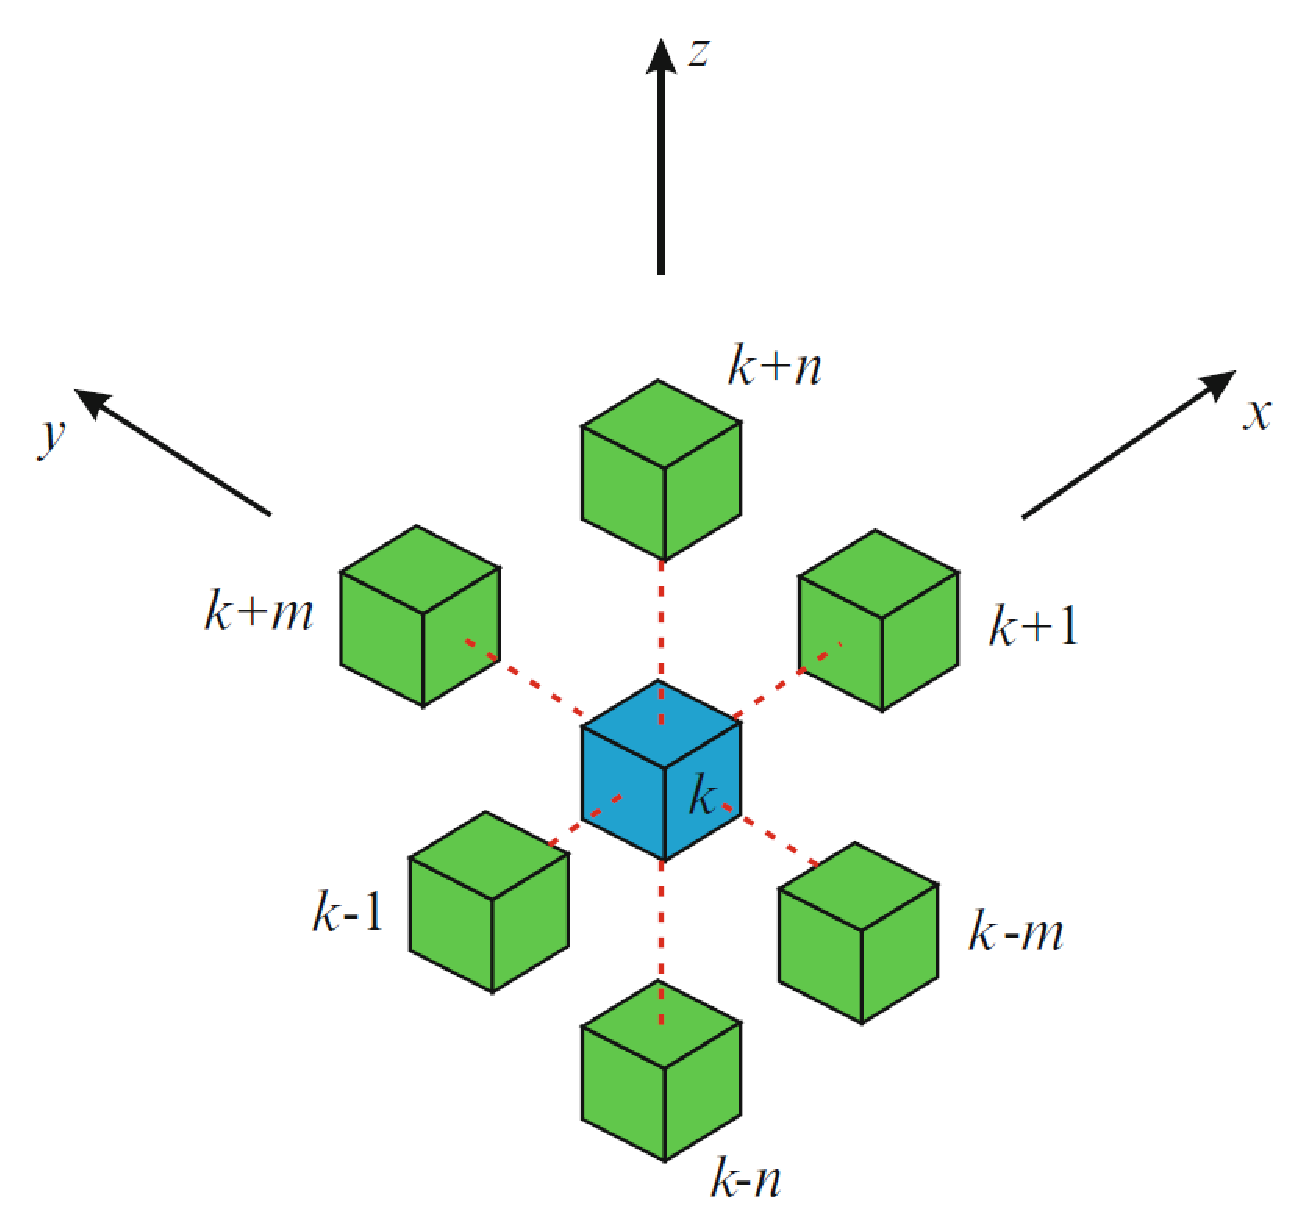
\includegraphics[width=0.5\linewidth]{chap/image/pdm_local}

  \caption{\label{pdm_local}
           局域性假设下的近场动力学。物质粒子 $\mathbf{x}$ 仅仅和$(k-l)$,$(k+l)$,$(k-m)$,$(k+m)$,$(k-n)$,和 $(k+n)$ 周围六个粒子相互作用。图片取自\mycite{Madenci}{2014}。
          }
\end{figure}

在局域性假设下,针对粒子 $k$,公式\ref{pdm_governing_function_discrete}则可以写成如下形式,
\begin{equation}
\rho_{(k)}\ddot{\mb{u}}_{(k)}
= \sum_{j=k-l,k+l,k-m,k+m,k-n,k+n}(\mb{t}_{(k)(j)}-\mb{t}_{(j)(k)})V_{(j)} + \mb{b}_{(k)}
\label{pdm_local_governing_function}
\end{equation}
这里 $\mb{t}_{(k)(j)}$ 表示物质粒子 $j$ 施加给物质粒子 $k$的内力密度,而 $\mb{t}_{(j)(k)}$ 表示物质粒子 $k$ 施加给物质粒子 $j$ 的内力密度。根据中心差分公式,经典连续介质力学中的本构方程(即公式\ref{fem_governing_function})可以写成分量形式,以 $x$ 分量为例,有

\begin{equation}
\begin{aligned}
\rho_{(k)}\ddot{\mb{u}}_{x(k)} &= \quad \frac{1}{2}\frac{\sigma_{xx(k)} - \sigma_{xx(k-l)}}{\Delta x} + \frac{1}{2}\frac{\sigma_{xx(k+l)} - \sigma_{xx(k)}}{\Delta x}\\
                              &\quad+  \frac{1}{2}\frac{\sigma_{xy(k)} - \sigma_{xy(k-m)}}{\Delta y} + \frac{1}{2}\frac{\sigma_{xy(k+m)} - \sigma_{xy(k)}}{\Delta y}\\
                              &\quad+  \frac{1}{2}\frac{\sigma_{zx(k)} - \sigma_{zx(k-n)}}{\Delta z} + \frac{1}{2}\frac{\sigma_{xz(k+n)} - \sigma_{xz(k)}}{\Delta z}\\
                              &\quad + \mb{b}_{x(k)}
\label{fem_local_governing_function}
\end{aligned}
\end{equation}
在上式中,每一项都仅仅和物质粒子 $k$ 以及直接邻居相关。我们可以将公式\ref{pdm_local_governing_function}写成类似的形式,即

\begin{equation}
\begin{aligned}
\rho_{(k)}\ddot{\mb{u}}_{(k)} &= \quad (\mb{t}_{(k)(k-l)} - \mb{t}_{(k-l)(k)})V_{(k-l)} + (\mb{t}_{(k)(k+l)} - \mb{t}_{(k+l)(k)})V_{(k+l)}\\
                             &\quad + (\mb{t}_{(k)(k-m)} - \mb{t}_{(k-m)(k)})V_{(k-m)} + (\mb{t}_{(k)(k+m)} - \mb{t}_{(k+m)(k)})V_{(k+m)}\\
                             &\quad + (\mb{t}_{(k)(k-n)} - \mb{t}_{(k-n)(k)})V_{(k-n)} + (\mb{t}_{(k)(k+n)} - \mb{t}_{(k+n)(k)})V_{(k+n)}\\
                             &\quad  + \mb{b}_{(k)}
\label{pdm_local_governing_function_2}
\end{aligned}
\end{equation}

通过比较方程 \ref{fem_local_governing_function} 和方程 \ref{pdm_local_governing_function_2},可以得到关于柯西应力和内力密度的关系,即

\begin{equation}
\sigma_{\alpha\beta(k)} = 2t_{\beta(k)(q_\alpha)}\Delta\alpha V_{(q_\alpha)}\qquad \mathrm{with } \quad q_x=(k+l),q_y=(k+m),q_z=(k+n)
\label{eq:7}
\end{equation}
\begin{equation}
\sigma_{\alpha\beta(k)} = -2t_{\beta(k)(q_\alpha)}\Delta\alpha V_{(q_\alpha)}\qquad \mathrm{with } \quad q_x=(k-l),q_y=(k-m),q_z=(k-n),
\label{eq:8}
\end{equation}

其中$\alpha,\beta=x,y,z$。对于正压力(normal stress),我们有

\begin{equation}
\sigma_{\alpha\alpha} = 2 \mb{t}_{(k)(q_\alpha)}\cdot(\mb{x}_{(q_\alpha)}-\mb{x}_{k})V_{(q_\alpha)}.
\label{eq:9}
\end{equation}

还可以进一步得到

\begin{equation}
\begin{aligned}
\sum_{\beta=x,y,z}\sigma_{\alpha\beta(k)}^2 &= \sum_{\beta=x,y,z}4t_{\beta(k)(q_\alpha)}^2(\Delta\alpha)^2 V_{(q_\alpha)}^2 \\
                                            &= 4(\mb{t}_{(k)(q_\alpha)}|\mb{x}_{(q_\alpha)}-\mb{x}_{k}|V_{(q_\alpha)})
                                                 \cdot
                                                (\mb{t}_{(k)(q_\alpha)}|\mb{x}_{(q_\alpha)}-\mb{x}_{k}|V_{(q_\alpha)}).
\end{aligned}
\label{eq:10}
\end{equation}

这一关系式将会在后续章节使用到。

\subsubsection{应变能量密度和内力密度}
在连续介质力学中,超弹性本构模型一般采用应变能量密度来进行表示(strain energy density),因此有必要建立应变能量密度和近场动力学中内力密度的关系。根据哈密顿力学理论,以及\mycite{Silling}{2007}关于 ordinary state-based 模型的定义,近场动力学中的内力密度可定义如下

\begin{equation}
\mb{t}_{(k)(j)}=\frac{1}{V_{(j)}}\frac{\partial W_{(k)}}{\partial (|\mb{y}_{(j)}-\mb{y}_{(k)}|)}\frac{\mb{y}_{(j)}-\mb{y}_{(k)}}{|\mb{y}_{(j)}-\mb{y}_{(k)}|},
\label{eq:11}
\end{equation}

其中 $W_{(k)}$ 表示物质粒子 $k$ 的应变能量密度。注意,力密度向量和物质粒子之间的连线方向是重合的,因而直接满足角动量守恒定律。上式可简写为
\begin{equation}
\mb{t}_{(k)(j)} = \frac{1}{2}A\frac{\mb{y}_{(j)}-\mb{y}_{(k)}}{|\mb{y}_{(j)}-\mb{y}_{(k)|}}
\label{eq:12}
\end{equation}
及
\begin{equation}
\mb{t}_{(j)(k)} = -\frac{1}{2}B\frac{\mb{y}_{(j)}-\mb{y}_{(k)}}{|\mb{y}_{(j)}-\mb{y}_{(k)|}},
\label{eq:13}
\end{equation}

其中$A$ 和 $B$ 是辅助变量,其形式取决于物质的材质参数,形变,以及邻域半径 $\delta$。

\subsubsection{超弹性模型通用推导框架}
给定连续介质力学中某一超弹性模型的应变能量表示,我们可以通过遵循相同的步骤来推得近场动力学中内力密度的具体形式。而一旦获得内力密度的显式形式,便可以进一步推导得到在近场动力学理论下的本构方程,从而进行后续的仿真工作。

对于一般模型的超弹性材质的推导步骤总结如下:
\begin{enumerate}
  \item 使用内力密度 $\mathbf{t}$ 来表示应变能量密度 $W$。通常而言,在连续介质力学中,应变能量密度通常通过应力张量 $\sigma$ 来进行表示,或者可以方便地转换为此种形式。然后通过应力张量 $\sigma$ 和内力密度 $\mathbf{t}$ 的关系(即\ref{eq:7} $\sim$ \ref{eq:10}),我们就可以直接建立应变能量密度 $W$ 和 $\mathbf{t}$ 之间的联系。
  \item 将 $\mathbf{t}$ (方程 \ref{eq:12}和\ref{eq:13})代入到能量密度 $W$ 的表达式,并根据式 \ref{eq:11} 执行微分操作,获得力密度 $\mathbf{t}$ 的具体形式。
  \item 在多种不同的简单受力情况下,通过比较连续介质力学中的应变能量密度以及近场动力学中对应的能量密度来确定相应的材质参数。选择的受力情况一般应尽量简单,并且是可以在连续介质力学和近场动力学中进行解析计算的。最后根据两种理论算得的能量应该相等,从而确定近场动力学中的材质参数。
\end{enumerate}

本文下面将通过线性弹性模型的推导来具体展示这一流程,这也是本文工作所用动力学模型。根据上述步骤,还可以推得其他超弹性模型在近场动力学理论中的表示,例如 FEM 中常用的不可压 Neo-Hookean 材质模型 \mycite{Bang}{2016}。

\subsubsection{线性弹性模型推导}
\noindent{\textbf{步骤1:使用内力密度表达应力能量密度}

对于连续介质力学中的各向同性线性弹性材料,关于物质粒子 $k$,应变能量密度 $W(k)$ 的具体形式可写为

\begin{equation}
W_{(k)} = \frac{\kappa}{2}\theta_{(k)}^2+\left[\frac{1}{4\mu}(\sigma_{xx(k)}^2+\sigma_{yy(k)}^2+\sigma_{zz(k)}^2)
                                         +\frac{1}{2\mu}(\sigma_{xy(k)}^2+\sigma_{xz(k)}^2+\sigma_{yz(k)}^2)
                                         -\frac{3\kappa^2}{4\mu}\theta_{(k)}^2
                                    \right],
\label{eq:14}
\end{equation}

其中 $\kappa$ 和 $\mu$ 的含义与前述章节一致,分别为体积模量和剪切模量。上式右边第一项衡量的是材质的各向均匀膨胀能量,而第二项衡量的是剪切能量。其中膨胀度 $\theta_{(k)}$(dilatation)被定义为

\begin{equation}
\theta_{(k)} = \epsilon_{xx(k)}+\epsilon_{yy(k)}+\epsilon_{zz(k)} = \frac{\sigma_{xx(k)}+\sigma_{yy(k)}+\sigma_{zz(k)}}{3\kappa}.
\label{eq:15}
\end{equation}

对式\ref{eq:14}稍微进行重整,则可以得到

\begin{equation}
\begin{aligned}
W_{(k)} =& \frac{\kappa}{2}\theta_{(k)}^2 -\frac{3\kappa^2}{4\mu}\theta_{(k)}^2 \\
         &+\frac{1}{8\mu}\left[(\sigma_{xx(k)}^2+\sigma_{xy(k)}^2+\sigma_{xz(k)}^2) + (\sigma_{xx(k)}^2+\sigma_{xy(k)}^2+\sigma_{xz(k)}^2)\right]\\
         &+\frac{1}{8\mu}\left[(\sigma_{yx(k)}^2+\sigma_{yy(k)}^2+\sigma_{yz(k)}^2) + (\sigma_{yx(k)}^2+\sigma_{yy(k)}^2+\sigma_{yz(k)}^2)\right]\\
         &+\frac{1}{8\mu}\left[(\sigma_{zx(k)}^2+\sigma_{zy(k)}^2+\sigma_{zz(k)}^2) + (\sigma_{zx(k)}^2+\sigma_{zy(k)}^2+\sigma_{zz(k)}^2)\right],
\end{aligned}
\label{eq:16}
\end{equation}

在上式中,关于应力张量的每一项被分别对应于粒子 $k$ 的六个直接邻居 $(k-l)$,$(k+l)$,$(k-m)$,$(k+m)$,$(k-n)$ 和 $(k+n)$。 使用式 \ref{eq:10} 建立的关系,即可得

\begin{equation}
\begin{aligned}
W_{(k)} =& (\frac{\kappa}{2} -\frac{3\kappa^2}{4\mu})\theta_{(k)}^2 \\
         &+\frac{1}{2\mu}\sum_{\substack {j=k-l,k+l,\\ \quad k-m,k+m,\\ \quad k-n,k+n}}(\mb{t}_{(k)(j)}|\mb{x}_{(j)}-\mb{x}_{(k)}|V_{(j)})\cdot(\mb{t}_{(k)(j)}|\mb{x}_{(j)}-\mb{x}_{(k)}|V_{(j)}).
\end{aligned}
\label{eq:17}
\end{equation}

同样可以将膨胀度 $\theta_{(k)}$ 写成分别对应六个邻居粒子的形式

\begin{equation}
\begin{aligned}
\theta_{(k)} =& \frac{\sigma_{xx(k)}+\sigma_{yy(k)}+\sigma_{zz(k)}}{3\kappa}\\
        =& \frac{1}{3\kappa}(\frac{1}{2}\sigma_{xx(k)}+\frac{1}{2}\sigma_{yy(k)}+\frac{1}{2}\sigma_{zz(k)}
         + \frac{1}{2}\sigma_{xx(k)}+\frac{1}{2}\sigma_{yy(k)}+\frac{1}{2}\sigma_{zz(k)}).
\end{aligned}
\label{eq:18}
\end{equation}

将式 \ref{eq:9} 代入上述方程, 则可以获得 $\theta_{(k)}$ 关于 $\mb{t}_{(k)}$ 的具体形式

\begin{equation}
\theta_{(k)} = \frac{1}{3\kappa}\left(\sum_{\substack {j=k-l,k+l,\\ \quad k-m,k+m,\\ \quad k-n,k+n}}(\mb{t}_{(k)(j)}\cdot(\mb{x}_{(j)}-\mb{x}_{(k)})V_{(j)})\right).
\label{eq:19}
\end{equation}

结合式 \ref{eq:17} 和式 \ref{eq:19},便可以通过内力密度 $\mb{t}_{(k)(j)}$ 来具体表示能量 $W_{(k)}$。

\noindent{\textbf{步骤2:获得力密度具体形式}

对于各向同性的线性弹性材料,物质粒子间的内力为线性关系,也就是其大小和 bond 之间的伸长度呈正比例关系。因此,内力密度 $\mb{t}_{(k)(j)}$ 可以写为更为具体的形式

\begin{equation}
\mb{t}_{(k)(j)} = \frac{1}{2}cs_{(k)(j)}\frac{\mb{y}_{(j)} - \mb{y}_{(k)}}{|\mb{y}_{(j)} - \mb{y}_{(k)}|},
\label{eq:20}
\end{equation}
其中
\begin{equation}
s_{(k)(j)} = \frac{|\mb{y}_{(j)} - \mb{y}_{(k)}| - |\mb{x}_{(j)} - \mb{x}_{(k)}|}{|\mb{x}_{(j)} - \mb{x}_{(k)}|}
\label{eq:21}
\end{equation}
为物质粒子间的伸长比例, $c$ 类似于质点弹簧系统中弹簧的弹性系数。

将式\ref{eq:20} 代入到式 \ref{eq:17} 和 \ref{eq:19},可得
\begin{equation}
\begin{aligned}
W_{(k)} =& (\frac{\kappa}{2} -\frac{3\kappa^2}{4\mu})\theta_{(k)}^2 \\
         &+\frac{c^2}{8\mu}\sum_{\substack {j=k-l,k+l,\\ \quad k-m,k+m,\\ \quad k-n,k+n}}(s_{(k)(j)}|\mb{x}_{(j)}-\mb{x}_{(k)}|V_{(j)})\cdot(s_{(k)(j)}|\mb{x}_{(j)}-\mb{x}_{(k)}|V_{(j)})
\end{aligned}
\label{eq:22}
\end{equation}
\begin{equation}
\theta_{(k)} = \frac{c}{6\kappa}\left(\sum_{\substack {j=k-l,k+l,\\ \quad k-m,k+m,\\ \quad k-n,k+n}}\left(s_{(k)(j)}\frac{\mb{y}_{(j)} - \mb{y}_{(k)}}{|\mb{y}_{(j)} - \mb{y}_{(k)}|}\cdot(\mb{x}_{(j)}-\mb{x}_{(k)})V_{(j)}\right)\right).
\label{eq:23}
\end{equation}

通过替换其中的常数系数,上述两式可以写为更一般化的形式

\begin{equation}
W_{(k)} = a\theta_{(k)}^2 + \sum_{\substack {j=k-l,k+l,\\ \quad k-m,k+m,\\ \quad k-n,k+n}}b(s_{(k)(j)}|\mb{x}_{(j)}-\mb{x}_{(k)}|V_{(j)})\cdot(s_{(k)(j)}|\mb{x}_{(j)}-\mb{x}_{(k)}|V_{(j)})
\label{eq:24}
\end{equation}
\begin{equation}
\theta_{(k)} = d\left(\sum_{\substack {j=k-l,k+l,\\ \quad k-m,k+m,\\ \quad k-n,k+n}}\left(s_{(k)(j)}\frac{\mb{y}_{(j)} - \mb{y}_{(k)}}{|\mb{y}_{(j)} - \mb{y}_{(k)}|}\cdot(\mb{x}_{(j)}-\mb{x}_{(k)})V_{(j)}\right)\right).
\label{eq:25}
\end{equation}
其中 $a$, $b$ 和 $d$ 为未决的动力学参数。

到目前为止,本文讨论的仍然在局域性假设下的近场动力学模型推导。可以通过直接扩充其作用半径,将这一模型应用到非局域的情形下,即
\begin{equation}
W_{(k)} = a\theta_{(k)}^2 + b\sum_{j=1}^{N}\omega_{(k)(j)}(s_{(k)(j)}|\mb{x}_{(j)}-\mb{x}_{(k)}|V_{(j)})\cdot(s_{(k)(j)}|\mb{x}_{(j)}-\mb{x}_{(k)}|V_{(j)})
\label{eq:26}
\end{equation}
\begin{equation}
\theta_{(k)} = d\sum_{j=1}^{N}\omega_{(k)(j)}s_{(k)(j)}\frac{\mb{y}_{(j)} - \mb{y}_{(k)}}{|\mb{y}_{(j)} - \mb{y}_{(k)}|}\cdot(\mb{x}_{(j)}-\mb{x}_{(k)})V_{(j)}.
\label{eq:27}
\end{equation}

其中$\sum_{\substack {j=k-l,k+l,\\ \quad k-m,k+m,\\ \quad k-n,k+n}}$ 被替换为 $\sum_{j=1}^{N}$,$N$ 表示在粒子 $k$ 邻域 $H_{\mb{x}}$ 中和其进行相互作用的粒子数量。此外,$\omega_{(k)(j)}$ 为权重函数,用来控制粒子 $k$ 对邻域内粒子的影响程度,定义为

\begin{equation}
\omega_{(k)(j)} = \frac{\delta}{|\mb{x}_{(j)}-\mb{x}_{(k)}|}.
\label{eq:28}
\end{equation}

注意 $\omega_{(k)(j)}$ 与方向无关,也就是模型是各向同性的。显而易见,当邻域内粒子离中心粒子 $k$ 越近时,则权重更大。利用式 \ref{eq:11} 所述内力密度定义,即可以获得 $\mb{t}_{(k)(j)}$ 的最终形式。

\begin{equation}
\mb{t}_{(k)(j)} = \frac{1}{2}A\frac{\mb{y}_{(j)} - \mb{y}_{(k)}}{|\mb{y}_{(j)} - \mb{y}_{(k)}|}
\label{eq:29}
\end{equation}
其中
\begin{equation}
A = 4\omega_{(k)(j)}\left\{ad\frac{\mb{y}_{(j)} - \mb{y}_{(k)}}{|\mb{y}_{(j)} - \mb{y}_{(k)}|}\cdot\frac{\mb{x}_{(j)} - \mb{x}_{(k)}}{|\mb{x}_{(j)} - \mb{x}_{(k)}|}\theta_{(k)}
   +b\left(|\mb{y}_{(j)} - \mb{y}_{(k)}| - |\mb{x}_{(j)} - \mb{x}_{(k)}|\right) \right\}.
\label{eq:30}
\end{equation}

\noindent{\textbf{步骤3:确定近场动力学参数}

在上节中,我们已经获取关于内力密度的表述式(\ref{eq:30}),仍其中存在三个未知的动力学参数($a, b, d$)需要确定。本节则通过两种简单的形变受力情况(各向均匀膨胀和简单剪切)来确认这些参数。\\

\noindent{\textit{Case 1: 各向均匀膨胀}}

各向均匀膨胀可以通过对材质各方向应用一个统一的应变 $\zeta$ 来实现,如图 \ref{pdm_isotropic_expansion} 所示。

\begin{figure}[htbp!]
  \centering
  \captionsetup{justification=centering}
  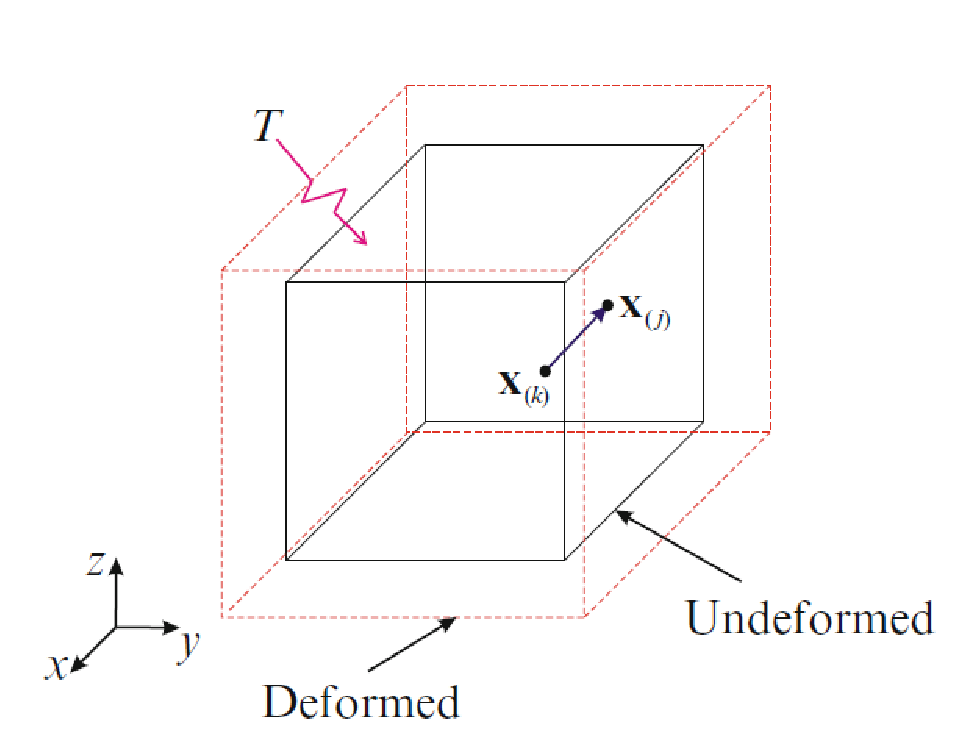
\includegraphics[width=0.5\linewidth]{chap/image/pdm_isotropic_expansion}

  \caption{\label{pdm_isotropic_expansion}
           各向均匀膨胀下的三维物体。图片取自\mycite{Madenci}{2014}。
          }
\end{figure}

在各向均匀膨胀下,应变张量为

\begin{eqnarray}
  \epsilon_{xx(k)} =  \epsilon_{yy(k)} = \epsilon_{zz(k)} = \zeta\\
  \epsilon_{xy(k)} =  \epsilon_{xz(k)} = \epsilon_{yz(k)} = 0
\end{eqnarray}

则经典连续介质力学中的应变能量密度 $W_{(k)}$ 和 膨胀度$\theta_{(k)}$ 可显式算得为

\begin{equation}
W_{(k)} = \frac{9}{2}\kappa\zeta^2\\
\label{eq:33}
\end{equation}
\begin{equation}
\theta_{(k)} = \epsilon_{xx(k)}+\epsilon_{yy(k)}+\epsilon_{zz(k)} = 3\zeta.
\label{eq:34}
\end{equation}

并且形变后的相对位置可用未形变空间的相对位置表示。即

\begin{equation}
|\mb{y}_{(j)} - \mb{y}_{(k)}| = (1+\zeta)|\mb{x}_{(j)} - \mb{x}_{(k)}|.
\label{eq:35}
\end{equation}

定义 $\bm{\xi} = \mb{x}_{(j)} - \mb{x}_{(k)}$, $\xi = |\bm{\xi}|$。
最终,$W_{(k)}$ 和 $\theta_{(k)}$ 的计算需要在半径为 $\delta$ 的圆球内进行积分:

\begin{equation}
\begin{aligned}
W_{(k)} =& a\theta_{(k)}^2
           +b\sum_{j=1}^{N}\omega_{(k)(j)}(s_{(k)(j)}|\mb{x}_{(j)}-\mb{x}_{(k)}|V_{(j)})\cdot(s_{(k)(j)}|\mb{x}_{(j)}-\mb{x}_{(k)}|V_{(j)})\\
        =& a\theta_{(k)}^2
           +b\int_0^\delta\int_0^{2\pi}\int_0^{\pi}\frac{\delta}{\xi}\left[(1+\zeta)\xi-\xi\right]^2\xi^2\sin(\phi)d\phi d\theta d\xi\\
        =& 9a\zeta^2+\pi b\delta^5\zeta^2
\end{aligned}
\label{eq:36}
\end{equation}
和
\begin{equation}
\begin{aligned}
\theta_{(k)} =& d\sum_{j=1}^{N}\omega_{(k)(j)}s_{(k)(j)}\frac{\mb{y}_{(j)} - \mb{y}_{(k)}}{|\mb{y}_{(j)} - \mb{y}_{(k)}|}\cdot(\mb{x}_{(j)}-\mb{x}_{(k)})V_{(j)}\\
        =& d\int_0^\delta\int_0^{2\pi}\int_0^{\pi}\frac{\delta}{\xi}\left[(1+\zeta)\xi-\xi\right](\frac{\bm{\xi}}{\xi}\cdot\frac{\bm{\xi}}{\xi})\xi^2\sin(\phi)d\phi d\theta d\xi\\
        =& \frac{4\pi d\delta^4}{3}\zeta,
\end{aligned}
\label{eq:37}
\end{equation}

其中 $(\xi,\theta,\phi)$ 为球坐标。将方程 \ref{eq:36}, \ref{eq:37}同方程\ref{eq:33}, \ref{eq:34}进行对比,则可以得到两个重要的关系式:

\begin{equation}
9a + \pi b\delta^5 = \frac{9}{2}\kappa
\label{eq:38}
\end{equation}
\begin{equation}
d = \frac{9}{4\pi\delta^4}.
\label{eq:39}
\end{equation}

\noindent{\textit{Case 2: 简单剪切}}

图\ref{pdm_simple_shear}所示为简单剪切形变下的三维物体。
\begin{figure}[htbp!]
  \centering
  \captionsetup{justification=centering}
  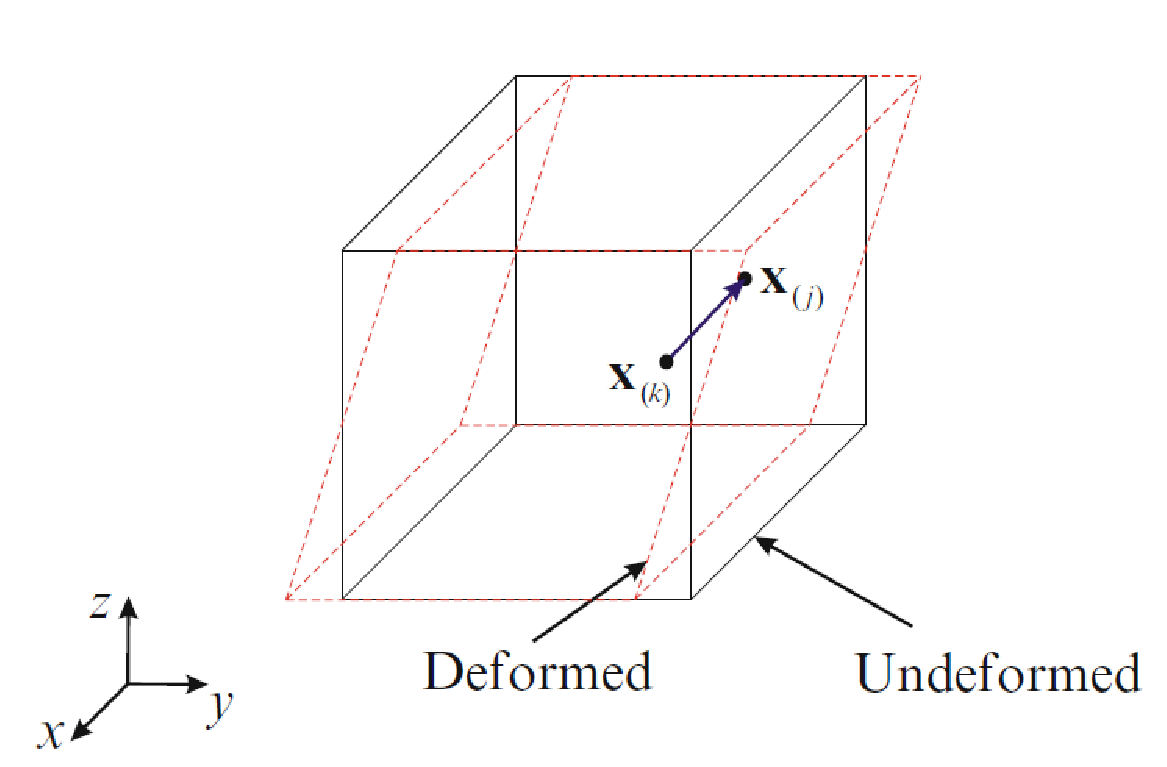
\includegraphics[width=0.5\linewidth]{chap/image/pdm_simple_shear}

  \caption{\label{pdm_simple_shear}
           简单剪切形变下的三维物体。图片取自\mycite{Madenci}{2014}。
          }
\end{figure}

在这种情形下,有类比关系:
\begin{equation}
\gamma_{xy(k)} = \zeta
\label{eq:40}
\end{equation}
\begin{equation}
\sigma_{xx(k)} = \sigma_{yy(k)} = \sigma_{zz(k)} = \gamma_{xz(k)} =\gamma_{yz(k)} = 0
\label{eq:41}
\end{equation}
及
\begin{equation}
|\mb{y}_{(j)} - \mb{y}_{(k)}| = (1+\frac{\zeta\sin(2\phi)\sin(\theta)}{2})|\mb{x}_{(j)} - \mb{x}_{(k)}|.
\label{eq:42}
\end{equation}

连续介质力学下的 $W_{(k)}$ 和 $\theta_{(k)}$ 则可以直接写为

\begin{equation}
W_{(k)} = \frac{1}{2}\mu\zeta^2\\
\label{eq:43}
\end{equation}
\begin{equation}
\theta_{(k)} = 0.
\label{eq:44}
\end{equation}

近场动力学下的 $W_{(k)}$ 的值仍然需要通过半径为 $\delta$ 的圆球内进行积分来计算。即
\begin{equation}
\begin{aligned}
W_{(k)} =& b\sum_{j=1}^{N}\omega_{(k)(j)}(s_{(k)(j)}|\mb{x}_{(j)}-\mb{x}_{(k)}|V_{(j)})\cdot(s_{(k)(j)}|\mb{x}_{(j)}-\mb{x}_{(k)}|V_{(j)})\\
        =& b\int_0^\delta\int_0^{2\pi}\int_0^{\pi}\frac{\delta}{\xi}\left[(1+\frac{\zeta\sin(2\phi)\sin(\theta)}{2})\xi-\xi\right]^2\xi^2\sin(\phi)d\phi d\theta d\xi\\
        =& \frac{b\pi\delta^5\zeta^2}{15}.
\end{aligned}
\label{eq:45}
\end{equation}

比较 \ref{eq:43} 和 \ref{eq:45} 获得:
\begin{equation}
b = \frac{15\mu}{2\pi\delta^5}.
\label{eq:46}
\end{equation}

将方程 \ref{eq:46} 代入 \ref{eq:38} 则可以获得 $a$ 的具体形式:
\begin{equation}
a = \frac{1}{2}(\kappa - \frac{5\mu}{3}).
\label{eq:47}
\end{equation}

到此为止,三个动力学参数($a, b, d$)已经全部确定。

\subsubsection{最终模型}

本章节已经推导了从经典连续介质力学到近场动力学理论,各向同性线性材料的本构模型的整个演变过程。为免读者混淆以及方便后续章节引用,在此我们做简要总结。在 ordinary state based 模型下,力密度的计算通过如下方式计算:

\begin{equation}
\tkj = \frac{1}{2}A\frac{\bfyj - \bfyk}{|\bfyj - \bfyk|}
\label{eq:48}
\end{equation}
其中
\begin{equation}
A = 4\wkj\left\{ad\frac{\bfyj-\bfyk}{|\bfyj-\bfyk|}\cdot\frac{\bfxj-\bfxk}{|\bfxj-\bfxk|}\thetak
   +b\left(|\bfyj - \bfyk| - |\bfxj - \bfxk|\right) \right\}
\label{eq:49}
\end{equation}
\begin{equation}
\thetak = d\sum_{j=1}^{N}\wkj\skj\frac{\bfyj - \bfyk}{|\bfyj - \bfyk|}\cdot(\bfxj-\bfxk)V_{(j)}
\label{eq:50}
\end{equation}
\begin{equation}
a = \frac{1}{2}(\kappa - \frac{5\mu}{3})
\label{eq:51}
\end{equation}
\begin{equation}
b = \frac{15\mu}{2\pi\delta^5}
\label{eq:52}
\end{equation}
\begin{equation}
d = \frac{9}{4\pi\delta^4}
\label{eq:53}
\end{equation}

